\documentclass[a4paper,12pt]{article} % тип документа

% Поля страниц
\usepackage[left=2.5cm,right=2.5cm,
    top=2cm,bottom=2cm,bindingoffset=0cm]{geometry}
    
%Пакет дял таблиц   
\usepackage{multirow}
\usepackage{longtable}
    
%Отступ после заголовка    
\usepackage{indentfirst}


% Рисунки
\usepackage{floatrow,graphicx,calc}
\usepackage{wrapfig}

% Создаёем новый разделитель
\DeclareFloatSeparators{mysep}{\hspace{1cm}}

% Ссылки?
\usepackage{hyperref}
\usepackage[rgb]{xcolor}
\hypersetup{				% Гиперссылки
    colorlinks=true,       	% false: ссылки в рамках
	urlcolor=blue          % на URL
}


%  Русский язык
\usepackage[T2A]{fontenc}			% кодировка
\usepackage[utf8]{inputenc}			% кодировка исходного текста
\usepackage[english,russian]{babel}	% локализация и переносы


% Математика
\usepackage{amsmath,amsfonts,amssymb,amsthm,mathtools, mathrsfs}


% Что-то 
\usepackage{wasysym}


\begin{document}
\begin{center}
	\footnotesize{ФЕДЕРАЛЬНОЕ ГОСУДАРСТВЕННОЕ АВТОНОМНОЕ ОБРАЗОВАТЕЛЬНОЕ 			УЧРЕЖДЕНИЕ ВЫСШЕГО ОБРАЗОВАНИЯ}\\
	\footnotesize{МОСКОВСКИЙ ФИЗИКО-ТЕХНИЧЕСКИЙ ИНСТИТУТ\\(НАЦИОНАЛЬНЫЙ 			ИССЛЕДОВАТЕЛЬСКИЙ УНИВЕРСИТЕТ)}\\
	\footnotesize{ФАКУЛЬТЕТ ОБЩЕЙ И ПРИКЛАДНОЙ ФИЗИКИ\\}
	\hfill \break
	\hfill\break
	\hfill\break
	\hfill \break
	\hfill \break
	\hfill \break
	\hfill \break
	\hfill \break
	\hfill \break
	\hfill \break
	\hfill \break
	\hfill \break
	\hfill \break
	\hfill \break
	\large{Лабораторная работа № 3.4.4\\\textbf{Петля гистерезиса (статический метод)}}\\
	\hfill \break
	\hfill \break
	\hfill \break
	\begin{flushright}
		Серебренников Даниил\\
		Группа Б02-826
	\end{flushright}
	\hfill \break
	\hfill \break
	\hfill \break
	\hfill \break
	\hfill \break
\end{center}
\hfill \break
\hfill \break
\hfill \break
\hfill \break
\hfill \break
\hfill \break
\begin{center}
	Долгопрудный, 2019 г.
\end{center}
\thispagestyle{empty}
\newpage

\textbf{Цель работы:} исследование кривых намагничивания ферромагнетиков с помощью баллистического гальванометра.

\textbf{В работе используются:} генератор токов намагничивания (ГТН), тороид, соленоид, баллистический гальванометр с осветителем и шкалой, мультиметр-амперметр, лабораторный автотрансформатор (ЛАТР), разделительный трансформатор, ключи, переключатели.


\section{Теоретическая часть}
	К ферромагнетикам принадлежат железо, никель, кобальт, гадолиний, их многочисленные сплавы с другими металлами. К ним примыкают ферриты -- диэлектрики со структурой антиферромагнетика.
	
	Ферромагнетики -- вещества, которые при определенной температуре обладают самопроизвольной намагниченностью $\boldsymbol{M}$ в отсутствие внешнего магнитного поля. В ферромагнетиках образуются отдельные намагниченные области – домены (от $10^{-2}$ до $10^{-6}$ см$^3$), магнитные моменты в которых ориентируются параллельно.
	
	Зависимость вектора магнитной индукции $\boldsymbol{B}$ ферромагнетика от вектора напряженности магнитного поля $\boldsymbol{H}$ нелинейна. В системе СИ эта связь имеет вид
	\begin{equation} \label{eq:BM}
		\boldsymbol{B} = \mu_0(\boldsymbol{H} + \boldsymbol{M})
	\end{equation}
	
	При циклическом перемагничивании зависимость (\ref{eq:BM}) изображается замкнутой кривой - симметричной петлей гистерезиса (рис. \ref{ris:hysteresis}), где $\pm \boldsymbol{H}_c$ – значение напряженности магнитного поля, необходимое для полного размагничивания ферромагнетика (коэрцитивная сила); $\pm \boldsymbol{B}_r$ – магнитная индукция, которую имеет ферромагнетик при напряженности внешнего магнитного поля, равную нулю (остаточная намагниченность); $\pm \boldsymbol{B}_s$ – значение магнитной индукции, при которой материал достигает насыщения (намагниченность насыщения)\footnote{Кривая, иозображающая зависимость $B(H)$, практически совпадает с зависимостью $M(H)$, поскольку второй член в выражении (\ref{eq:BM}), в малых полях, существенно превосходит первый}.
	\begin{figure}[H]
		\center{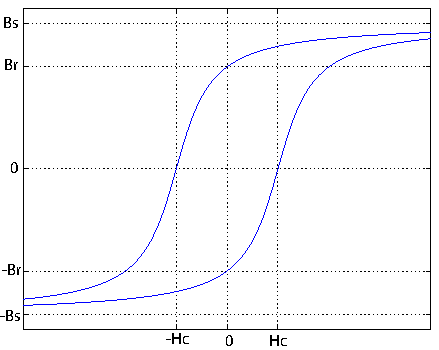
\includegraphics[scale=1]{hysteresis.pdf}}
		\caption{Петля гистерезиса ферромагнетика.}
		\label{ris:hysteresis}
	\end{figure}

\newpage
\section{Экспериментальная установка}
	\begin{figure}[H]
		\center{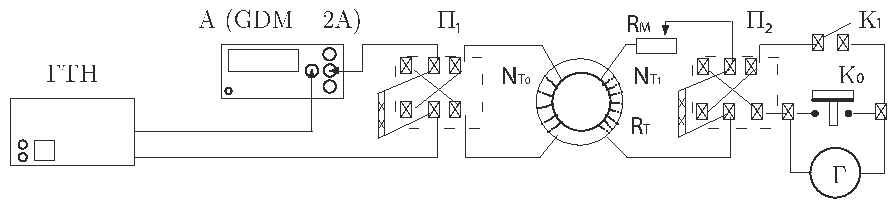
\includegraphics[scale=1]{ustanovka_1.pdf}}
		\caption{Схема установки для исследования петли гистерзеиса.}
		\label{ris:ustanovka_1}
	\end{figure}
	\begin{figure}[H]
		\center{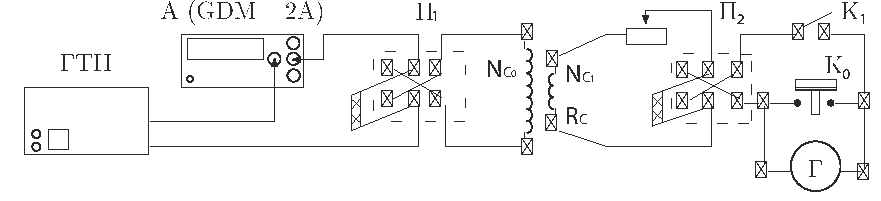
\includegraphics[scale=1]{ustanovka_2.pdf}}
		\caption{Схема установки для калибровки гальванометра.}
		\label{ris:ustanovka_2}
	\end{figure}
	\begin{figure}[H]
		\center{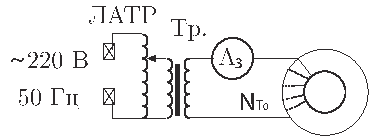
\includegraphics[scale=1]{ustanovka_3.pdf}}
		\caption{Схема установки для размагничивания образца.}
		\label{ris:ustanovka_3}
	\end{figure}

	\begin{itemize}
		\item
			Напряженность магнитного поля $H$ в тороиде зависит от тока, текущего в намагничивающей обмотке:
			\begin{equation}\label{eq:H}
				H = \frac{N_{T_0}}{\pi D} I;
			\end{equation}
		\item
			Связь между отклонением зайчика баллистического гальванометра в делениях $\Delta x$ и изменением магнитной индукции $\Delta B$ в сердечнике тороида:
			\begin{equation}\label{eq:B}
				\Delta B = \mu_0 \left(\frac{d_C}{d_T}\right)^2 \frac{N_{C_0}}{N_{T_1}} \frac{N_{C_1}}{l_C} \Delta I_1 \frac{\Delta x}{\Delta x_1}.
			\end{equation}
	\end{itemize}
	


\section{Экспериментальные данные}

		
	\floatsetup[table]{capposition=top}	
	\begin{table}[H]
		\caption{Параметры установки.}
		\label{table:const}
		\begin{tabular}{|c|c|c|c|c|c|c|c|}
			\hline
			$N_{T_0}$ & $N_{T_1}$ & $N_{C_0}$ & $N_{C_1}$ & $D$, м & $d_C$, см & $d_T$, см & $l_C$, м \\ \hline
			1750      & 300       & 940       & 500       & 0,1    & 7         & 1         & 0,8      \\ \hline
		\end{tabular}
	\end{table}


	\floatsetup[table]{capposition=top}	
	\begin{table}[H]
		\caption{Некоторые измеряемые величины и их погрешность.}
		\label{table:error}
		\begin{tabular}{|c|c|c|}
			\hline
			& $I$, мА & $\Delta x$, мм \\ \hline
			Величина          & 100     & 100            \\ \hline
			Погрешность       & 2       & 1,0            \\ \hline
			$\varepsilon$, \% & 2       & 1              \\ \hline
		\end{tabular}
	\end{table}


	\floatsetup[table]{capposition=top}	
	\begin{table}[H]
		\caption{Каллибровка гальванометра.}
		\label{table:calc}
		\begin{tabular}{|c|c|}
			\hline
			$\Delta I_1$, мА & $\Delta x_1$ \\ \hline
			1706             & 171          \\ \hline
		\end{tabular}
	\end{table}

	
	\begin{longtable}[c]{|c|c|c|c|c|}
		\caption[lot]{Данные предельной петли.}
		\label{table:limit}\\
		\hline
		$I$, мА & $\Delta x$, мм & $H$, А/м & $\Delta B$, Тл & $B$, Тл \\ \hline
		1705    & 66             & 9498     & 0,079          & -       \\ \hline
		1206    & 60             & 6718     & 0,072          & 1,30    \\ \hline
		869     & 62             & 4841     & 0,075          & 1,23    \\ \hline
		622     & 61             & 3465     & 0,073          & 1,15    \\ \hline
		434     & 32             & 2418     & 0,039          & 1,08    \\ \hline
		350     & 20             & 1950     & 0,024          & 1,04    \\ \hline
		303     & 12             & 1688     & 0,014          & 1,02    \\ \hline
		275     & 9              & 1532     & 0,011          & 1,00    \\ \hline
		253     & 9              & 1409     & 0,011          & 0,99    \\ \hline
		233     & 9              & 1298     & 0,011          & 0,98    \\ \hline
		213     & 10             & 1187     & 0,012          & 0,97    \\ \hline
		192     & 10             & 1070     & 0,012          & 0,96    \\ \hline
		171     & 29             & 953      & 0,035          & 0,95    \\ \hline
		121     & 38             & 674      & 0,046          & 0,91    \\ \hline
		60      & 45             & 334      & 0,054          & 0,87    \\ \hline
		0       & 59             & 0        & 0,071          & 0,81    \\ \hline
		-60     & 110            & -334     & 0,132          & 0,74    \\ \hline
		-121    & 71             & -674     & 0,085          & 0,61    \\ \hline
		-172    & 46             & -958     & 0,055          & 0,52    \\ \hline
		-193    & 64             & -1075    & 0,077          & 0,47    \\ \hline
		-214    & 71             & -1192    & 0,085          & 0,39    \\ \hline
		-234    & 88             & -1303    & 0,106          & 0,31    \\ \hline
		-254    & 107            & -1415    & 0,129          & 0,20    \\ \hline
		-276    & 147            & -1537    & 0,177          & 0,07    \\ \hline
		-304    & 255            & -1693    & 0,307          & -0,11   \\ \hline
		-350    & 280            & -1950    & 0,337          & -0,41   \\ \hline
		-434    & 243            & -2418    & 0,292          & -0,75   \\ \hline
		-621    & 95             & -3459    & 0,114          & -1,04   \\ \hline
		-868    & 103            & -4835    & 0,124          & -1,16   \\ \hline
		-1205   & 84             & -6712    & 0,101          & -1,28   \\ \hline
		-1705   & -60            & -9498    & -0,072         & -1,38   \\ \hline
		-1205   & -60            & -6712    & -0,072         & -1,31   \\ \hline
		-868    & -61            & -4835    & -0,073         & -1,24   \\ \hline
		-621    & -61            & -3459    & -0,073         & -1,16   \\ \hline
		-434    & -32            & -2418    & -0,039         & -1,09   \\ \hline
		-350    & -19            & -1950    & -0,023         & -1,05   \\ \hline
		-303    & -12            & -1688    & -0,014         & -1,03   \\ \hline
		-275    & -10            & -1532    & -0,012         & -1,01   \\ \hline
		-254    & -9             & -1415    & -0,011         & -1,00   \\ \hline
		-233    & -9             & -1298    & -0,011         & -0,99   \\ \hline
		-213    & -9             & -1187    & -0,011         & -0,98   \\ \hline
		-192    & -10            & -1070    & -0,012         & -0,97   \\ \hline
		-172    & -28            & -958     & -0,034         & -0,96   \\ \hline
		-121    & -38            & -674     & -0,046         & -0,92   \\ \hline
		-60     & -45            & -334     & -0,054         & -0,88   \\ \hline
		0       & -60            & 0        & -0,072         & -0,82   \\ \hline
		60      & -113           & 334      & -0,136         & -0,75   \\ \hline
		121     & -69            & 674      & -0,083         & -0,62   \\ \hline
		171     & -48            & 953      & -0,058         & -0,53   \\ \hline
		192     & -62            & 1070     & -0,075         & -0,47   \\ \hline
		213     & -72            & 1187     & -0,087         & -0,40   \\ \hline
		233     & -90            & 1298     & -0,108         & -0,31   \\ \hline
		254     & -108           & 1415     & -0,130         & -0,21   \\ \hline
		275     & -144           & 1532     & -0,173         & -0,08   \\ \hline
		303     & -265           & 1688     & -0,319         & 0,10    \\ \hline
		350     & -267           & 1950     & -0,321         & 0,42    \\ \hline
		434     & -247           & 2418     & -0,297         & 0,74    \\ \hline
		621     & -94            & 3459     & -0,113         & 1,04    \\ \hline
		868     & -102           & 4835     & -0,123         & 1,15    \\ \hline
		1205    & -84            & 6712     & -0,101         & 1,27    \\ \hline
		1705    & -              & 9498     & -              & 1,37    \\ \hline
	\end{longtable}
	

	\begin{table}[H]
		\caption{Данные начальной кривой намагничивания.}
		\label{table:start}
		\begin{tabular}{|c|c|c|c|c|}
			\hline
			$I$, мА & $\Delta x$, мм & $H$, А/м & $\Delta B$, Тл & $B$, Тл \\ \hline
			0       & 26             & 0,0      & 0,031          & 0       \\ \hline
			61      & 50             & 339,8    & 0,060          & 0,03    \\ \hline
			123     & 55             & 685,2    & 0,066          & 0,09    \\ \hline
			174     & 14             & 969,3    & 0,017          & 0,16    \\ \hline
			195     & 44             & 1086,2   & 0,053          & 0,17    \\ \hline
			216     & 33             & 1203,2   & 0,040          & 0,23    \\ \hline
			236     & 46             & 1314,6   & 0,055          & 0,27    \\ \hline
			257     & 48             & 1431,6   & 0,058          & 0,32    \\ \hline
			278     & 62             & 1548,6   & 0,075          & 0,38    \\ \hline
			306     & 104            & 1704,5   & 0,125          & 0,45    \\ \hline
			361     & 206            & 2010,9   & 0,248          & 0,58    \\ \hline
			436     & 188            & 2428,7   & 0,226          & 0,83    \\ \hline
			623     & 106            & 3470,4   & 0,128          & 1,05    \\ \hline
			865     & 104            & 4818,4   & 0,125          & 1,18    \\ \hline
			1205    & 86             & 6712,4   & 0,103          & 1,31    \\ \hline
			1705    &  -              & 9497,6   &    -            & 1,41    \\ \hline
		\end{tabular}
	\end{table}

		
\newpage
\section {Обработка результатов}
	Используя формулы (\ref{eq:H}) и (\ref{eq:B}) рассчитаем $H = f_1(I)$ и $\Delta B = f_2 (\Delta x)$ для начальной и предельной петель гистерезиса. По полученным данным (табл.\ref{table:limit}-\ref{table:start}) построим петлю гистерезиса $B = f (H)$. Стоит отметить, что для выполнения естественного условия $f(0) = 0$, к нашим результатам была прибавлена величина $B_0 = 1,38$ Тл. 
	\begin{figure}[H]
		\center{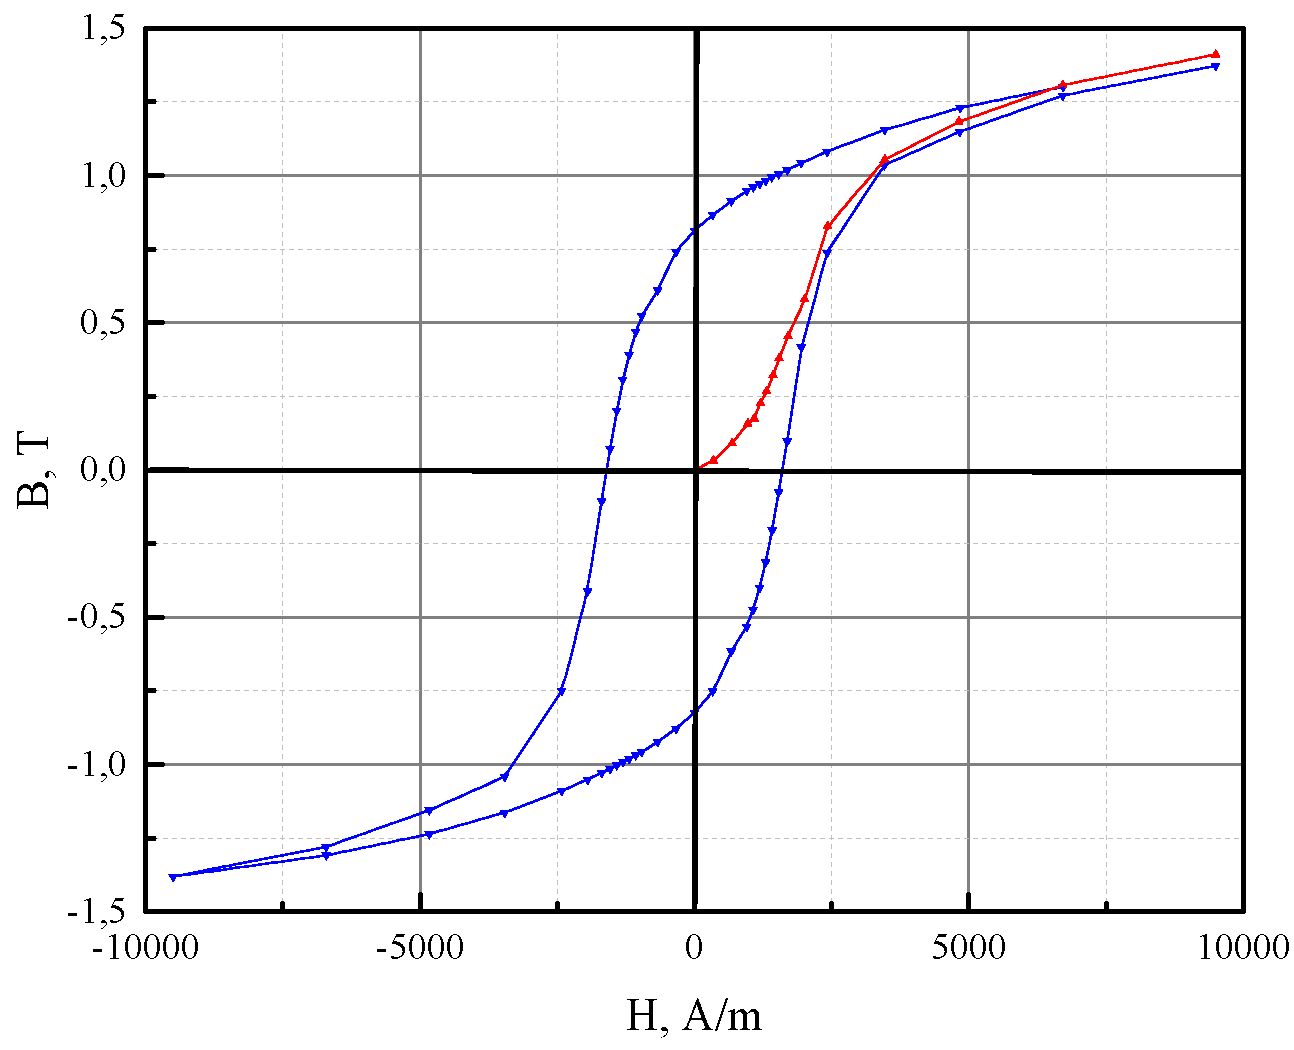
\includegraphics[scale=0.5]{plot.pdf}}
		\caption{Зависимость $B = f(I)$.}
		\label{ris:B=f(I)}
	\end{figure}


	По графику найдём коэрцитивную силу $H_c$, индукцию насыщения $B_s$ и остаточную индукцию $B_r$. Более того, можно вычислить максимальное значение дифференциальной магнитной проницаемости $\mu$ для начальной кривой намагничивания.
	\begin{table}[H]
		\caption{Анализ петли гистерезиса.}
		\label{table:result}
		\begin{tabular}{|c|c|c|c|}
			\hline
			$H_C$, А/м   & $B_S$, Тл         & $B_r$, Тл    & $\mu_{диф}$  \\ \hline
			$1600\pm 11$ & $1,410 \pm 0,010$ & $0,810\pm 0,010$ & $470 \pm 20$ \\ \hline
		\end{tabular}
	\end{table}

\section {Обсуждение результатов}
	В ходе данной лабоораторной работы мы исследовали кривую намагничивания стали с помощью баллистического гальванометра. Стоит отметить, что тороид во время эксперимента достаточно сильно нагревался, что могло спровоцировать переход материала в парамагнитное состояние при достижении точки Кюри. Однако для различных сплавов стали критическая температура довольно высока $T_c \approx 500$~К и не может быть достигнута вследствие рассеивания тепла, выделяемого токами в витках. Построенный график (рис.~\ref{ris:B=f(I)}) представляет собой симметричную петлю гистерезиса, что соответствует теории ферромагнетизма.
	
	Анализ петли гистерезиса стали показал, что коэрцитивная сила $H_c$ равна 1600 А/м с точностью в 0.8\%. Обратившись к техническо-инженерным справочникам, можно предположить, что наш образец состоит примерно на 2-6\% из Cr, на 0,6\% из C, на 4-8\% из W и на 40-42\% из Co -- такой сплав стали называется высококобальтовым. Для него характерна высокая остаточная индукция -- 1,10 Тл, что на 26\% больше нашего результата в 0,81 Тл. В связи с сильной зависимостью магнитных свойств сплава от его компонент вполне возможно, что наш образец имеет коэрцитивную силу, равную 1600 А/м, но при этом не является высококобальтовым.
	
	
\section{Выводы}
	\begin{enumerate}
		\item 
			Вычислили коэрцитивную силу $H_c = (1600\,\pm\, 11)$ А/м;
		\item 
			Определили остаточную индукцию: $B_r =(0,81\,\pm\,0,01)$ Тл и индукцию насыщения $B_s = (1,41\,\pm\, 0,01)$ Тл;
		\item
			Рассчитали максимальную дифференциальную магнитную проницаемость для начальной кривой намагничивания: $\mu = 470 \, \pm \, 20$;
		\item 	
			Состав сплава стали определить не удалось.
	\end{enumerate}








\end{document}